\mysection{結果}
\subsection{実験1}
実験 (2) の結果について、 DCモードの波形と比べてACモードの波形が全体的に画面の縦軸方向に移動した。
実験 (4) の結果について、トリガレベルが測定波形の正・負のピーク値の間にある時、波形が表示され、トリガレベルを負から正の値に動かすと、波形が全体的に横軸方向に動き、逆にトリガレベルを正から負の値に動かすと波形が全体的に横軸の逆方向に動いた。また、波形の外にトリガレベルを動かすと、波形が横軸方向に揺れ動いて表示された。
実験 (5) の結果について、正・負のピーク値の間にトリガレベルがあるとき、波形が表示され、トリガレベルを負から正、正から負に動かした場合の表示波形の変化は上記 (2) の結果に等しい。しかし、波形の外にトリガレベルを動かすと表示画面上方に小さく “ Ready ” の文字が表示され、波形の線が薄くなった。また、薄くなった線はファンクションジェネレータの電源をOFFにしても消えなかった。
実験 (6) の結果について、ディジタルオシロスコープの波形取り込みモードがサンプルのときと比べて、アベレージモードに変えると、波形の線が細くなった。
実験 (7) の結果について、 50 msの区間において5周期分の波形が観測されたため、\\
  \begin{equation*}
    \frac{5}{5.0\times10^{-2}} = 100 \si{[Hz]}
  \end{equation*}
よって、100 \si{[Hz]}である。
実験 (10) の結果について、サンプリング間隔を求めるために用いたデータを表\ref{tb2}に示す。
  \begin{table}[ht]
    \centering
    \caption{サンプリング間隔を求めるために用いたデータ (抜粋)}
    \begin{tabular}[t]{rr}
    \toprule
    \multicolumn{1}{c}{経過時間 \textit{t} \si{[s]}}&\multicolumn{1}{c}{オシロスコープの出力電圧 \si{[V]}}\\
    \midrule
    0&0.224\\
    0.000001&0.224\\
    0.000002&0.224\\
    0.000003&0.224\\
    0.000004&0.224\\
    0.000005&0.224\\
    0.000006&0.224\\
    0.000007&0.224\\
    0.000008&0.224\\
    0.000009&0.224\\
    \bottomrule
    \end{tabular}
    \label{tb2}
  \end{table}

  表\ref{tb2}において、サンプリング間隔が左の列が時間間隔を表すデータの、連続する上下のデータ同士の間隔であるため、その間隔は、\textbf{0.0000001} \si{[s]}である。
また、量子化間隔は右の列の連続する上下のデータ同士の間隔であるため、その間隔は、\textbf{20} \si{[mV]}である。
なお、この波形を観測したとき、\textbf{\textgt{水平軸レンジ}}: \textbf{0.000025} \si{[s]}、 \textbf{\textgt{垂直レンジ}}: \textbf{500} \si{[mV]}であった。

\mysubsection{実験2}

  数値積分の計算結果の有効数字について、式\eqref{eq5}の計算において、標本化された関数の和と時間間隔との積で、標本化された関数の末位は小数第3位であるため、標本化された関数の和は、最小桁を小数第3位とする。
  次に、標本化された関数の和と時間間隔との積について、関数の和の位取りは3桁で、時間間隔の位取りは7桁であるため、積の誤差を考慮し、意味のある数字のみを残すため、位取りの少ない方に有効桁を合わせるので、式\eqref{eq5}の計算結果の有効数字を3桁とする。表\ref{tb3}, \ref{tb4}に実験 (12) の結果を示す。(単位\si{V})
  
  \begin{table}[h]
    \begin{center}
      \begin{tabular}{cc}
        \begin{minipage}{0.45\textwidth}
          \centering
          \caption{フーリエ級数$b_n$について}
          \begin{tabular}[t]{rr}
            \toprule
            \multicolumn{1}{c}{$b_n$}&\multicolumn{1}{c}{フーリエ級数の値 \si{[V]}}\\
            \midrule
            $b_0$&0.0712\\
            $b_1$&-0.117\\
            $b_2$&0.0641\\
            $b_3$&-0.00722\\
            $b_4$&-0.0261\\
            $b_5$&0.0270\\
            $b_6$&-0.007\\
            \bottomrule
          \end{tabular}
          \label{tb3}
        \end{minipage}
        \begin{minipage}{0.4\textwidth}
          \centering
          \caption{フーリエ級数$a_n$について}
          \begin{tabular}[t]{rr}
            \toprule
            \multicolumn{1}{c}{$a_n$}&\multicolumn{1}{c}{フーリエ級数の値 \si{[V]}}\\
            \midrule
            $a_1$&0.217\\
            $a_2$&0.0988\\
            $a_3$&0.000504\\
            $a_4$&0.0586\\
            $a_5$&0.0353\\
            $a_6$&0.00114\\
            \bottomrule
          \end{tabular}
          \label{tb4}
        \end{minipage}
      \end{tabular}
    \end{center}
\end{table}

実験 (13) の結果について、近似波形、$b_0$に関する波形、被測定波形を図\ref{im5} \verb|~| 図\ref{im6} に示す。(図\ref{im6}は$n = 6$におけるフーリエ級数展開を式\ref{eq2} \verb|~| \ref{eq4} に適用。)

\begin{figure}[H]
  \begin{center}
    \subfigure[フーリエ級数による近似 ($n = 3$まで)]{
      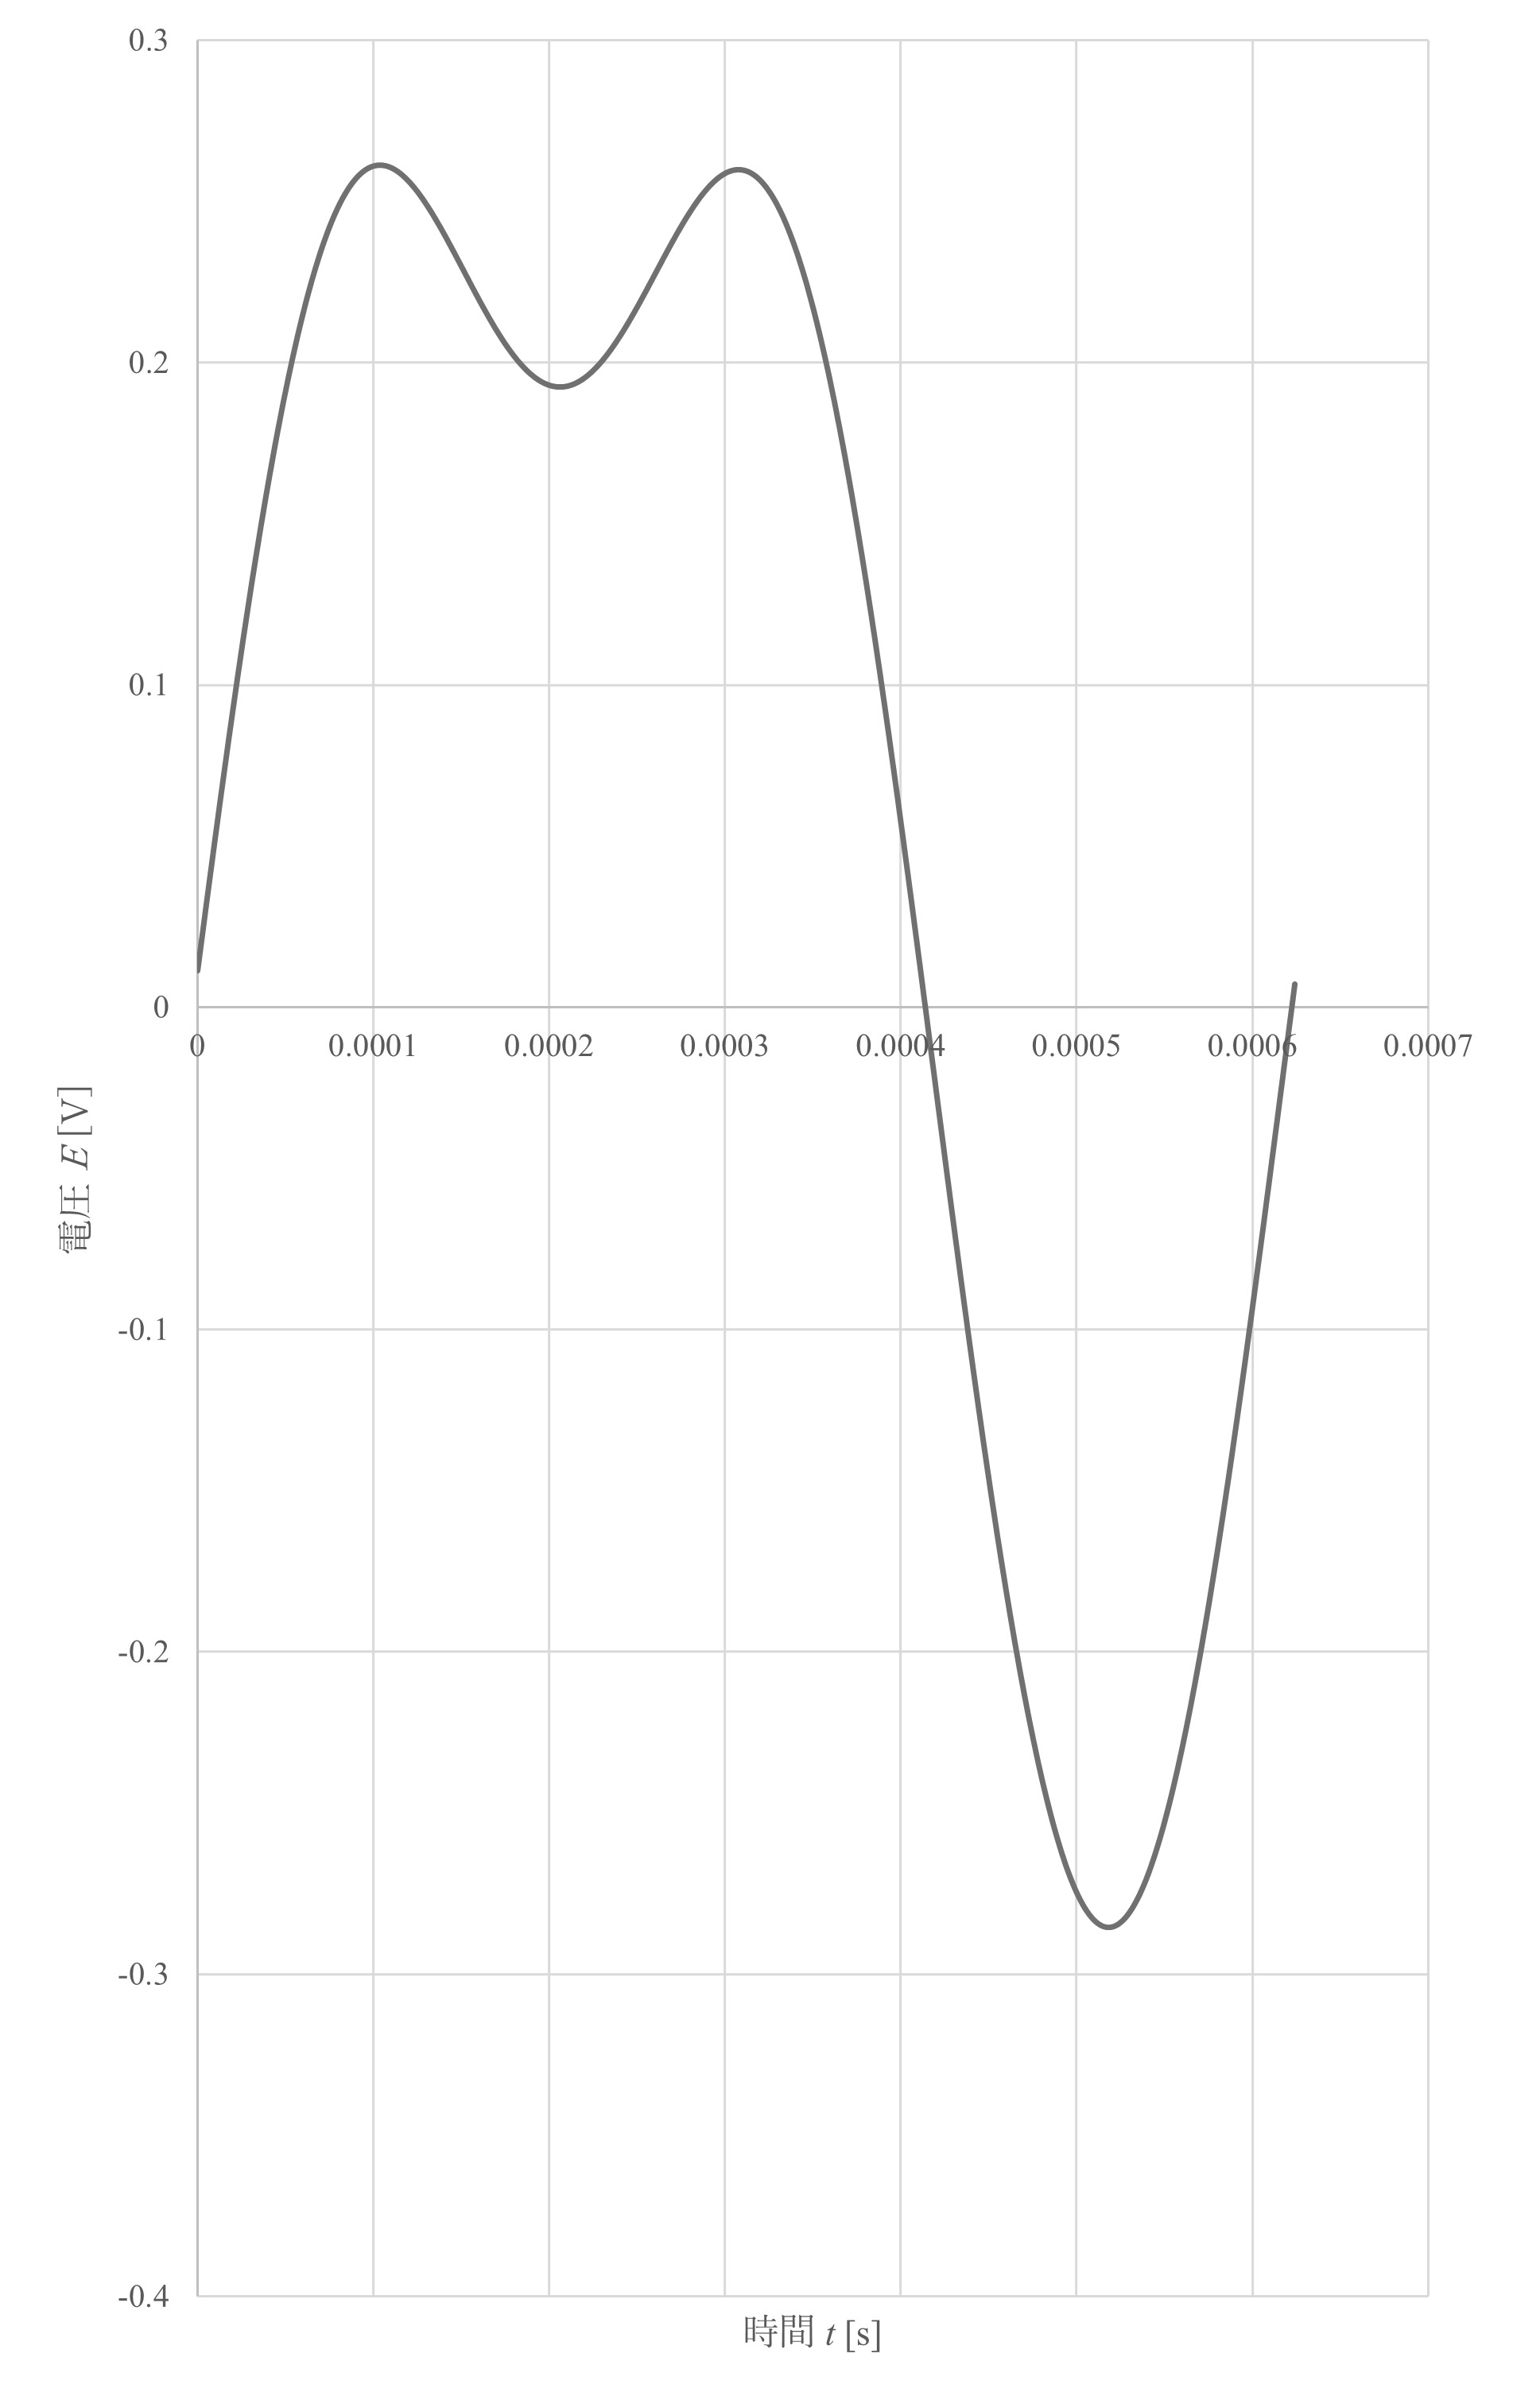
\includegraphics[width=.4\columnwidth]{img/5.jpg}
      \label{sub1}
    }~
    \subfigure[フーリエ級数による近似 ($n = 4$まで)]{
    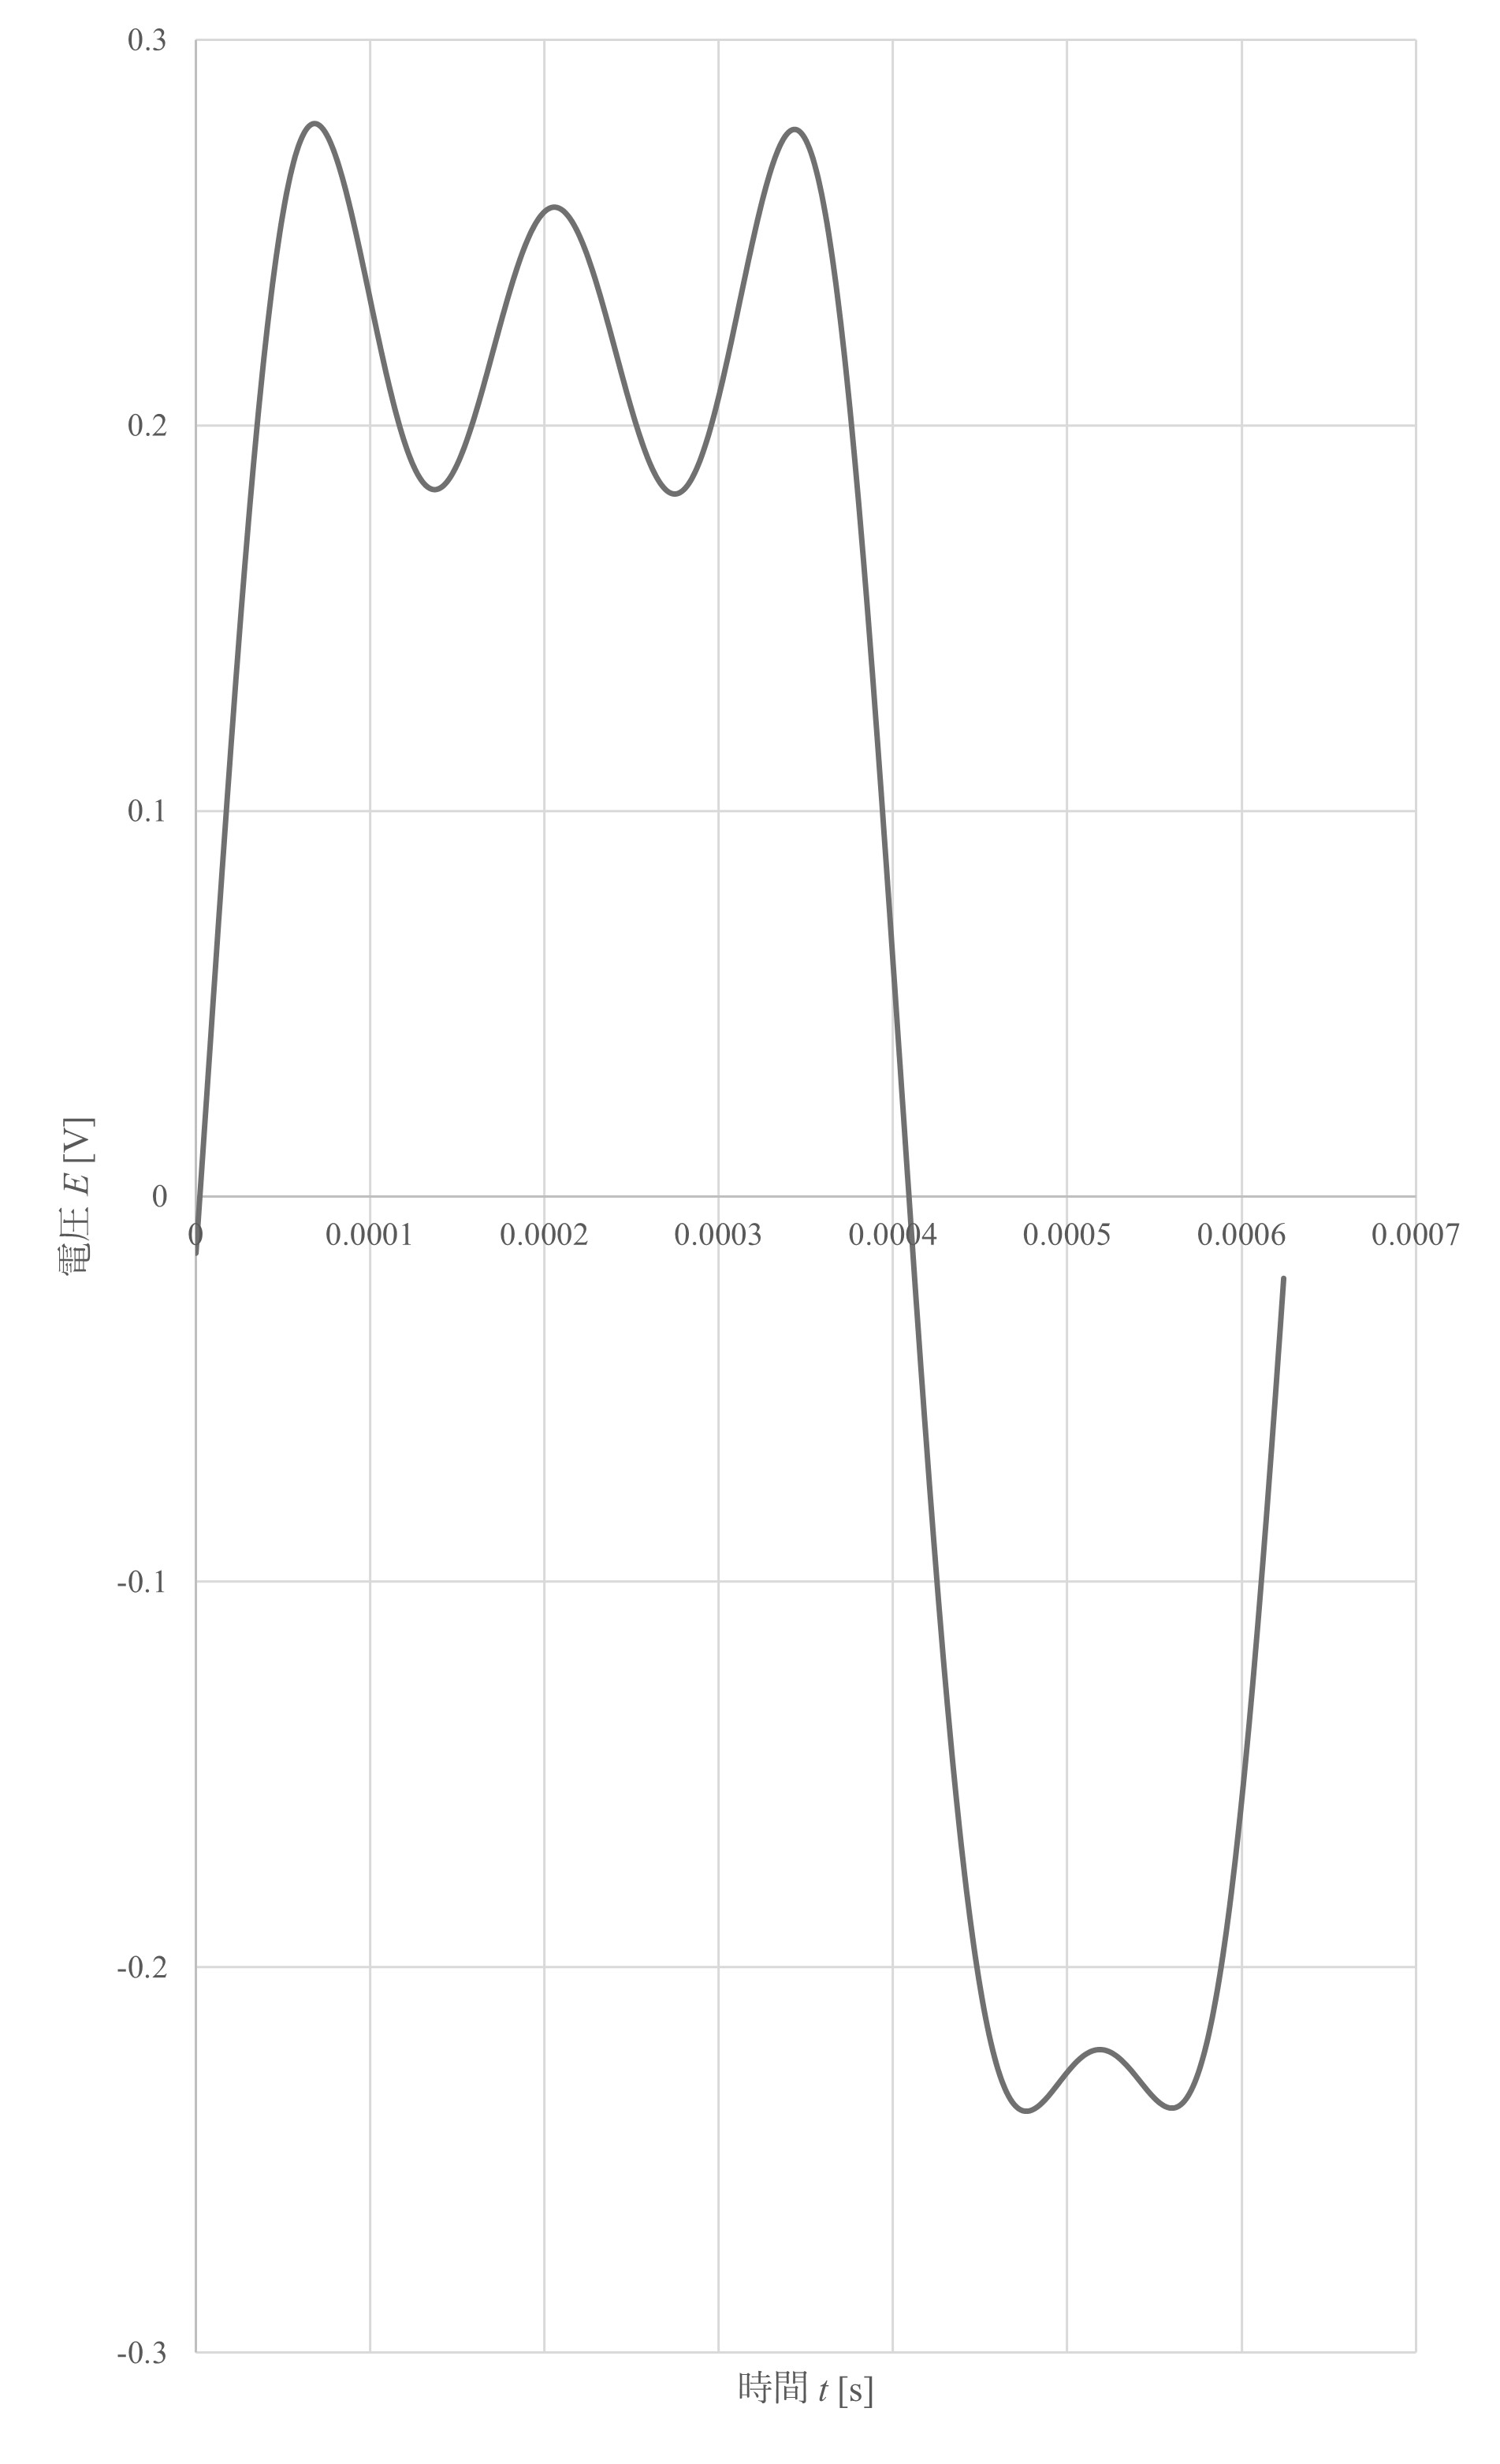
\includegraphics[width=.4\columnwidth]{img/6.jpg}
      \label{sub2}
    }
    \subfigure[フーリエ級数による近似 ($n = 5$まで)]{
    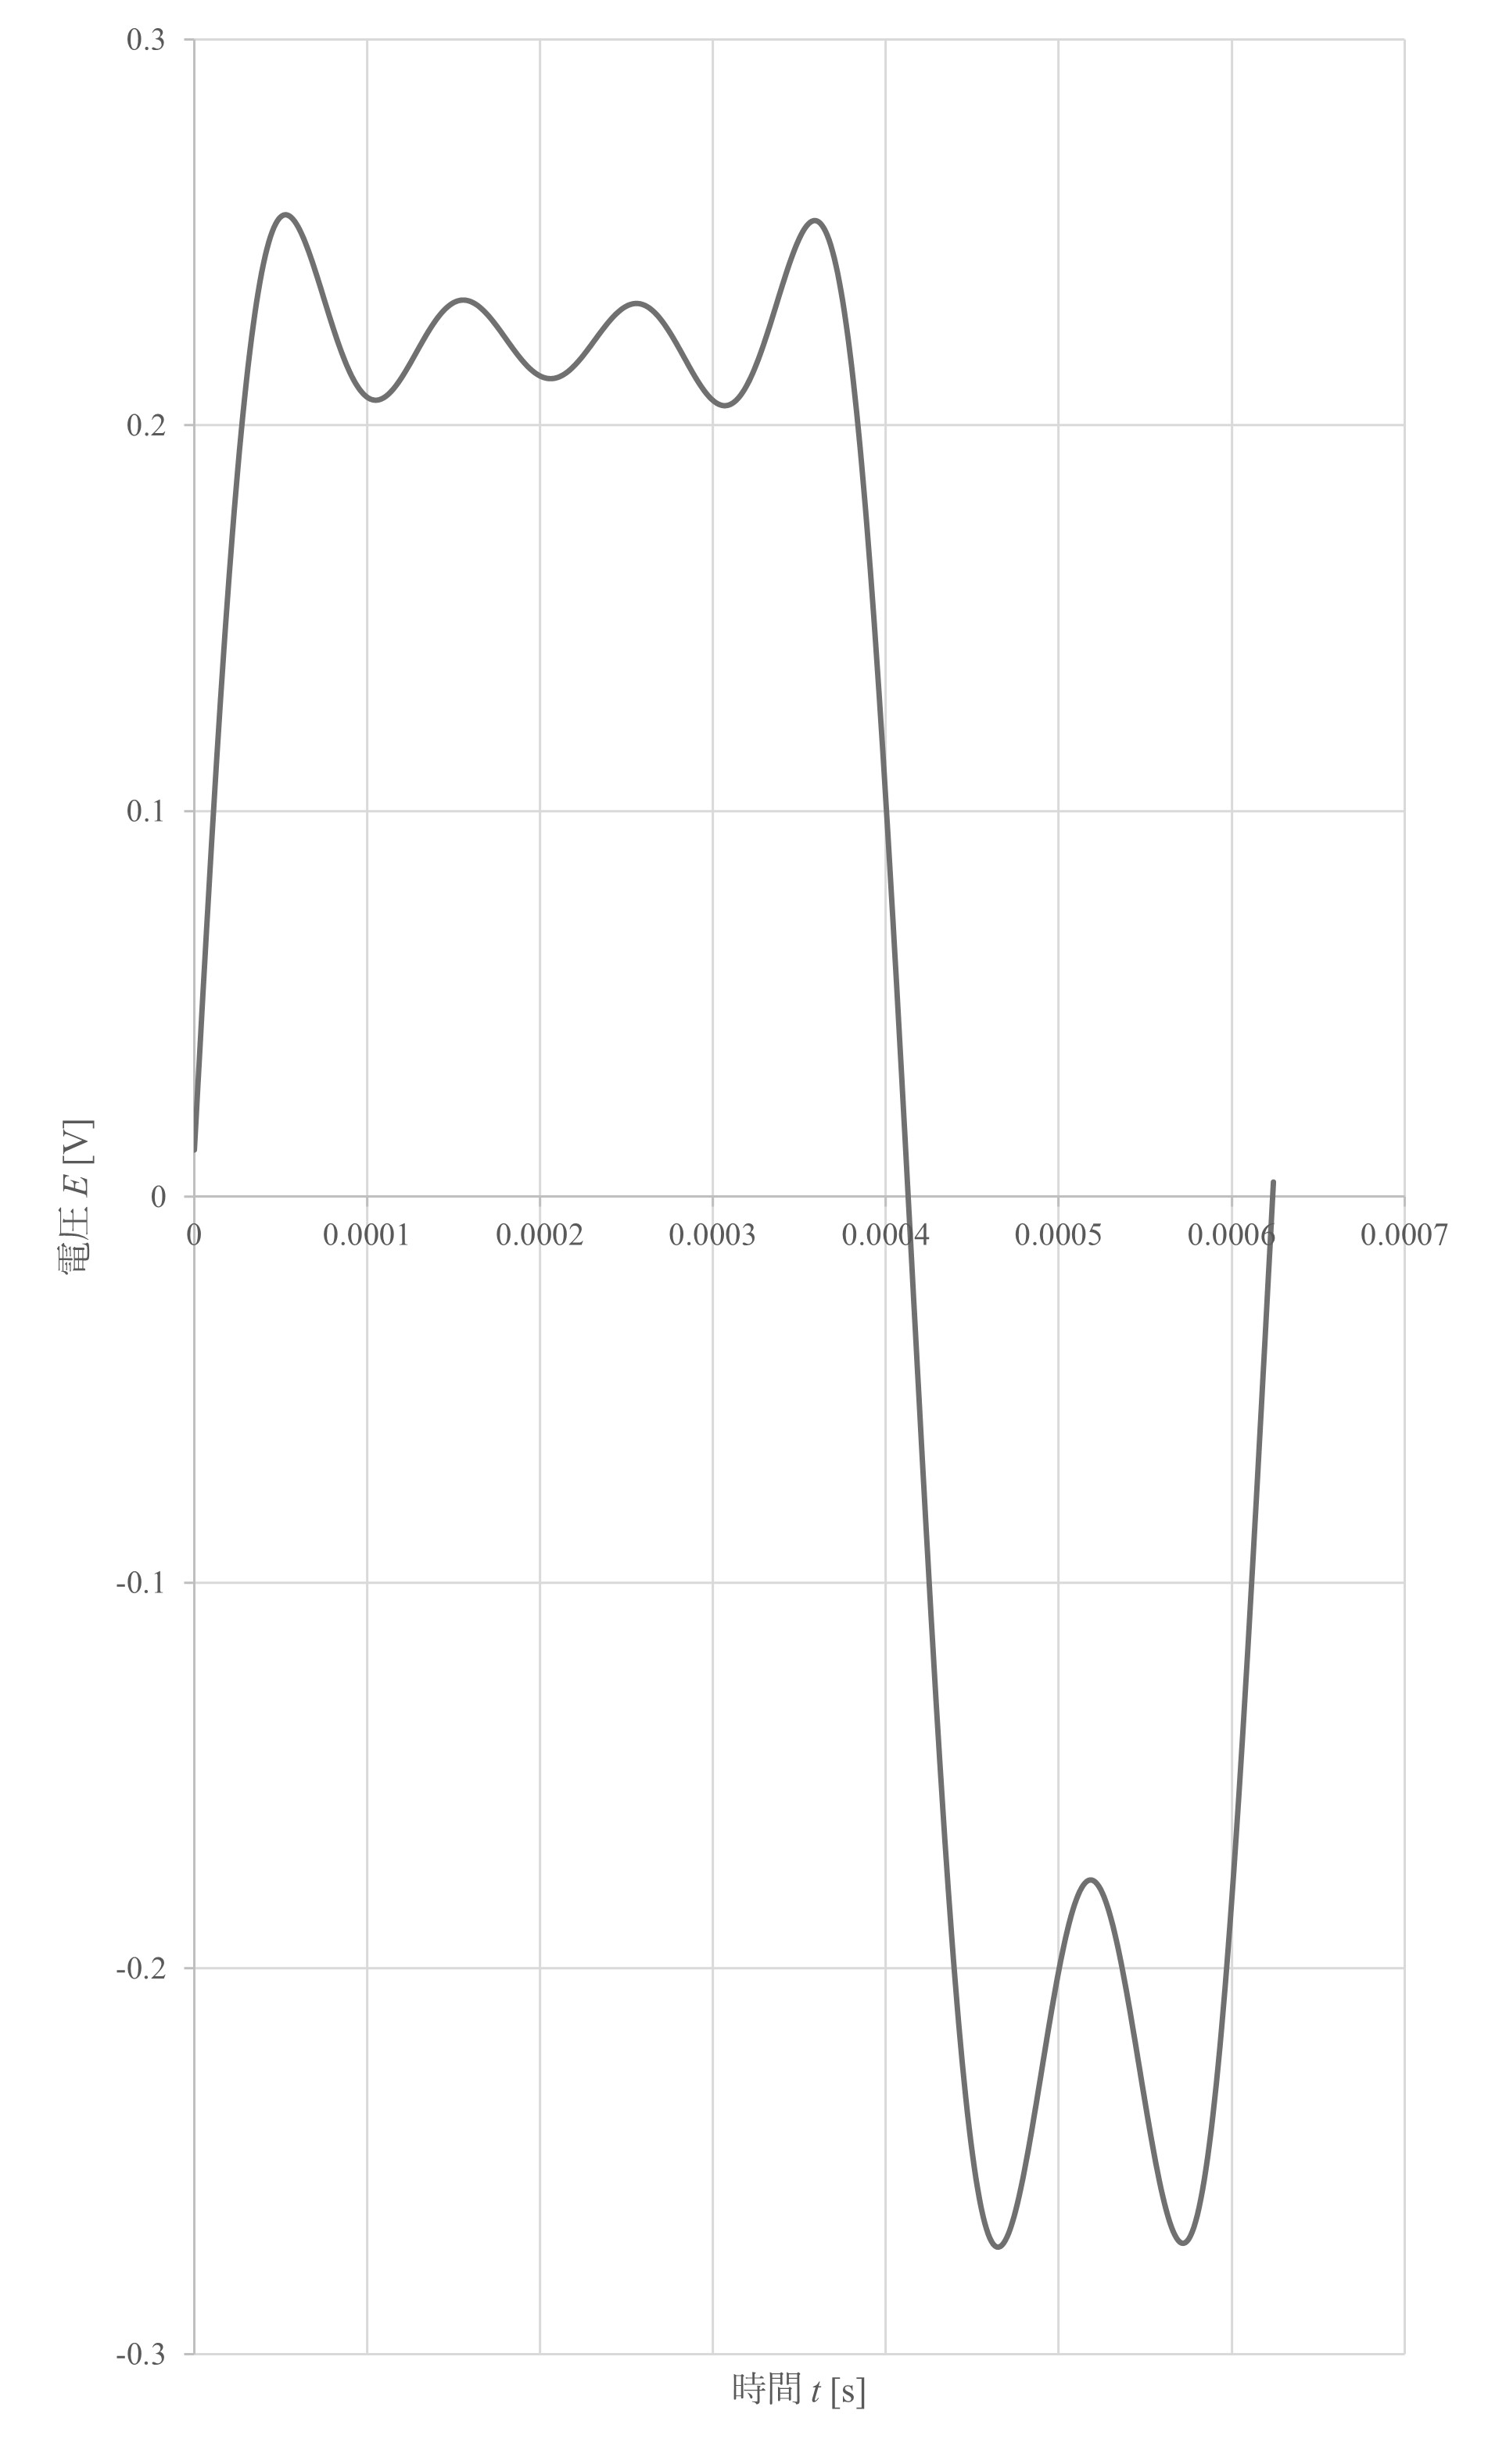
\includegraphics[width=.4\columnwidth]{img/7.jpg}
      \label{sub3}
    }~
    \subfigure[フーリエ級数による近似 ($n = 6$まで)]{
    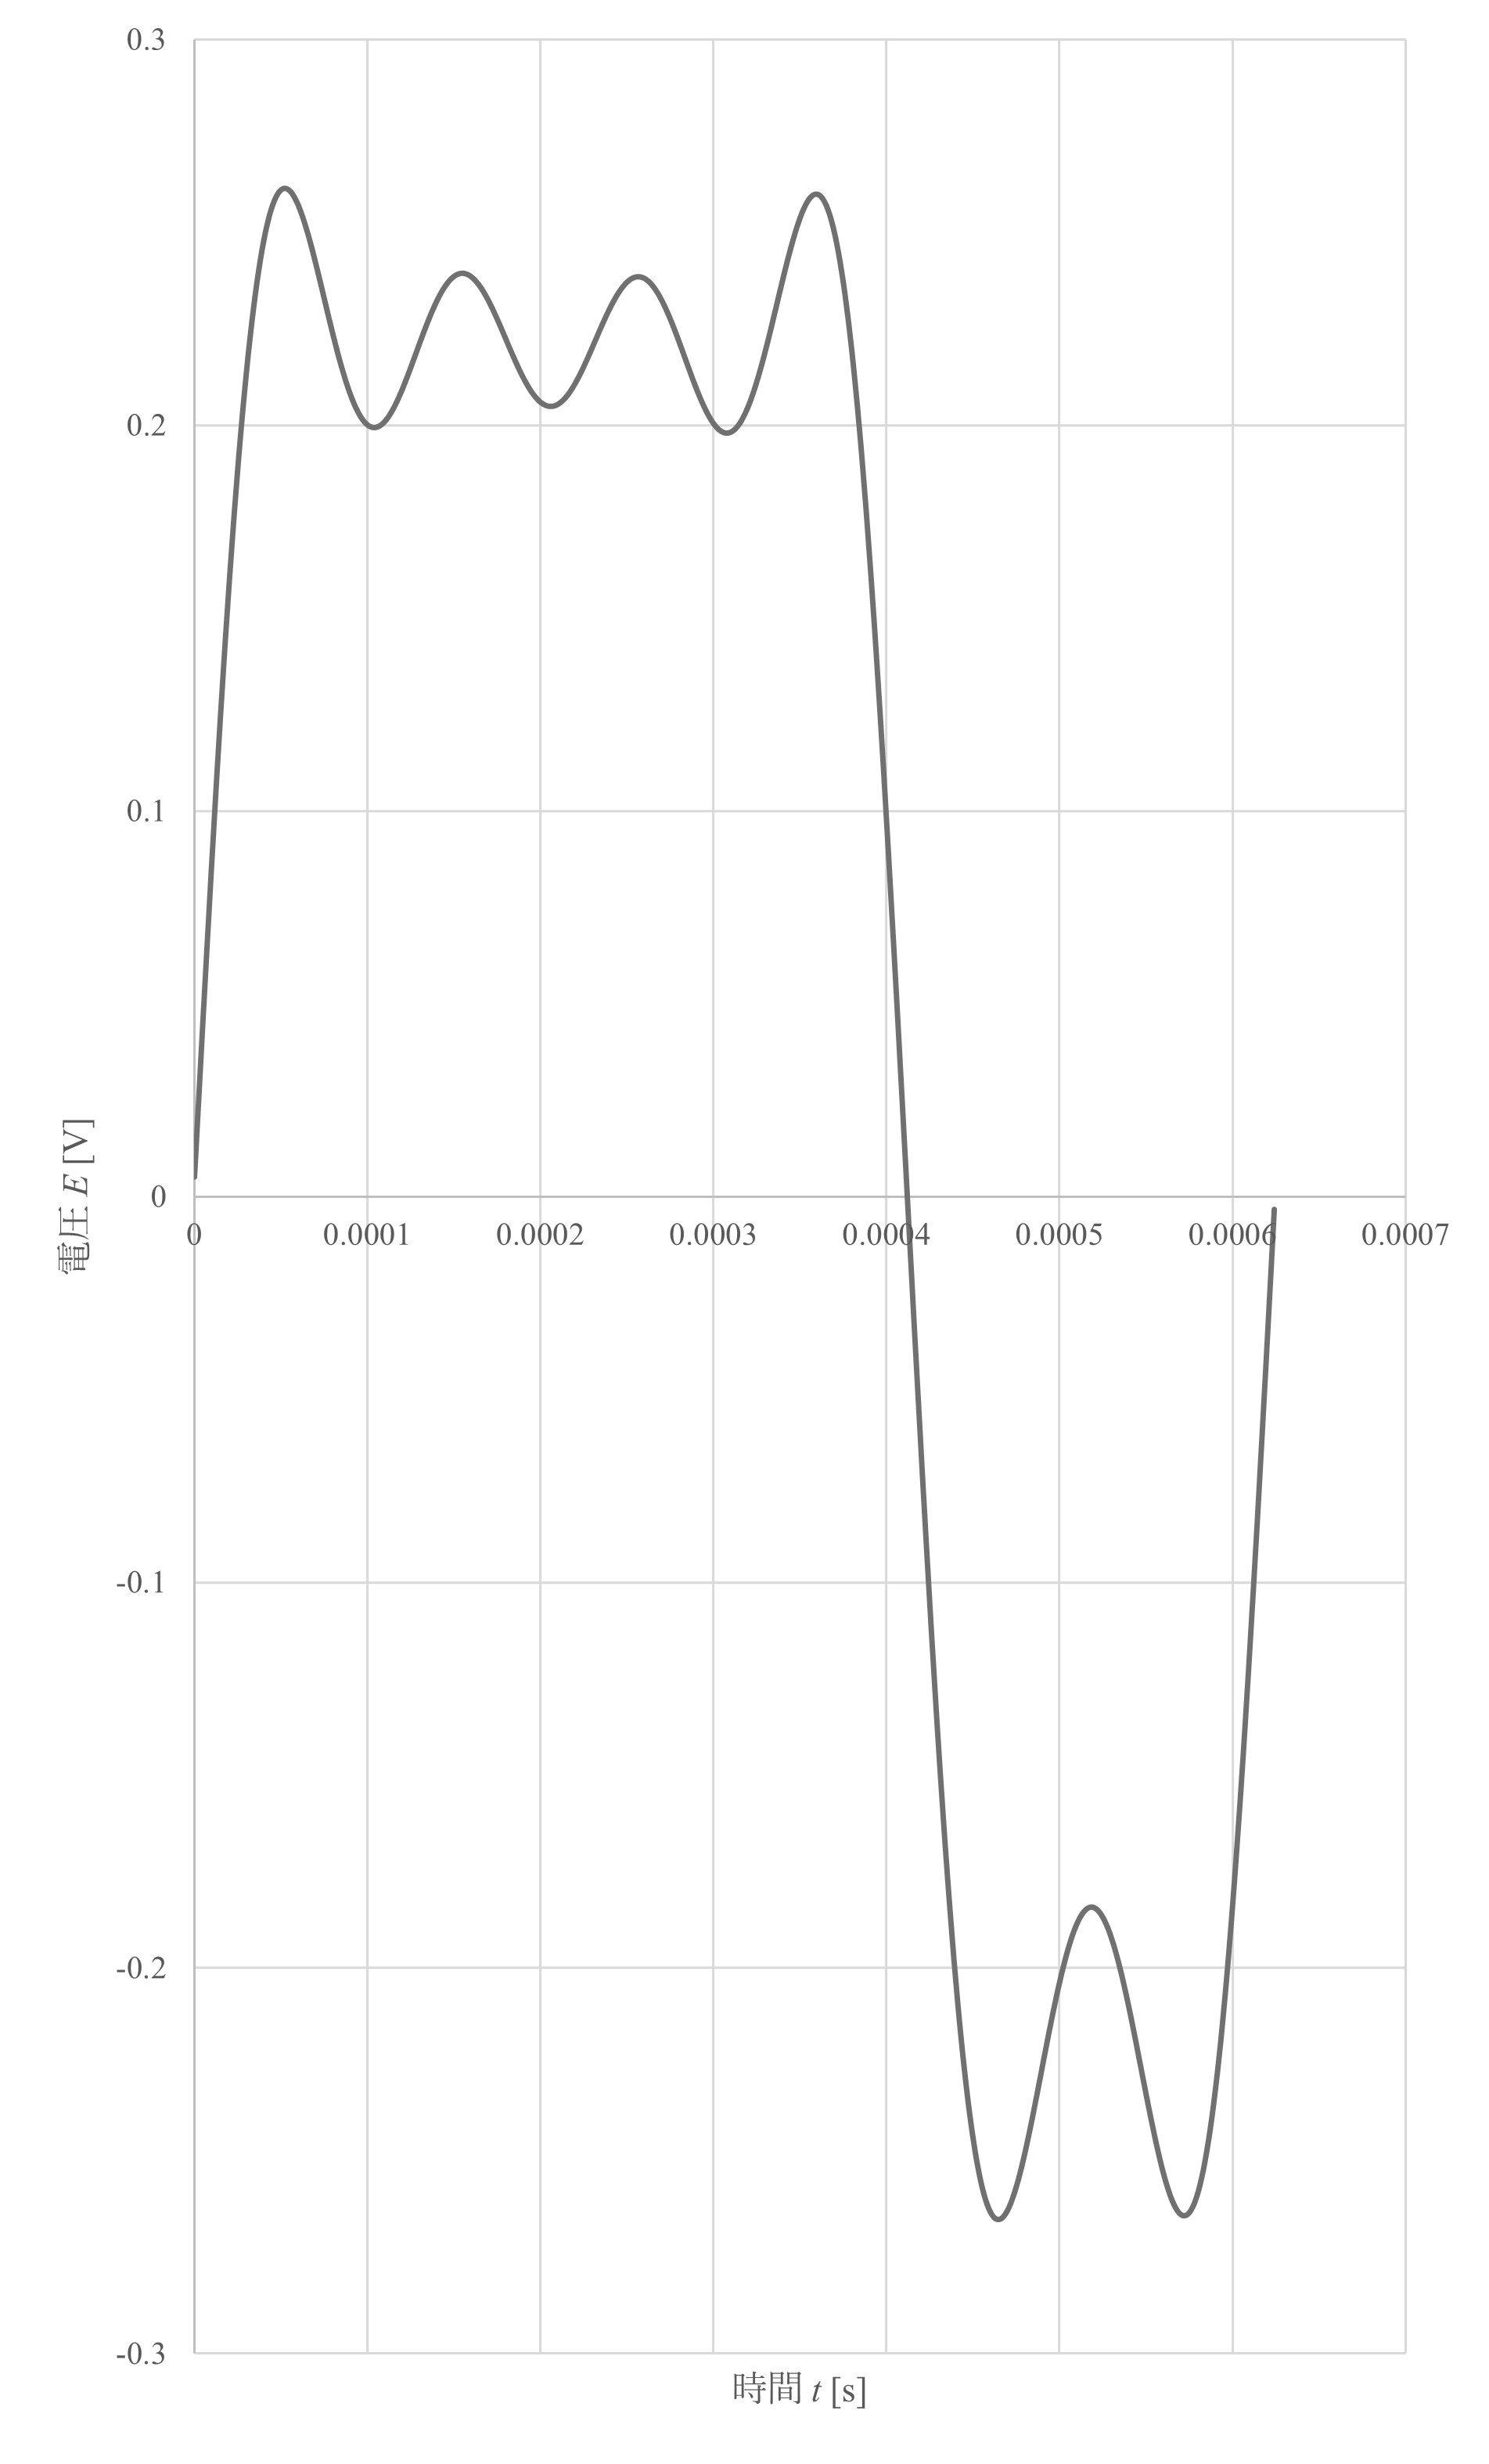
\includegraphics[width=.4\columnwidth]{img/8.jpg}
      \label{sub4}
    }
   \caption{フーリエ級数による近似}
   \label{im5}
   \end{center}
\end{figure}

\begin{figure}[H]
  \begin{center}
    \subfigure[$b_0$を足さずに計算した近似値($n = 6$まで)]{
      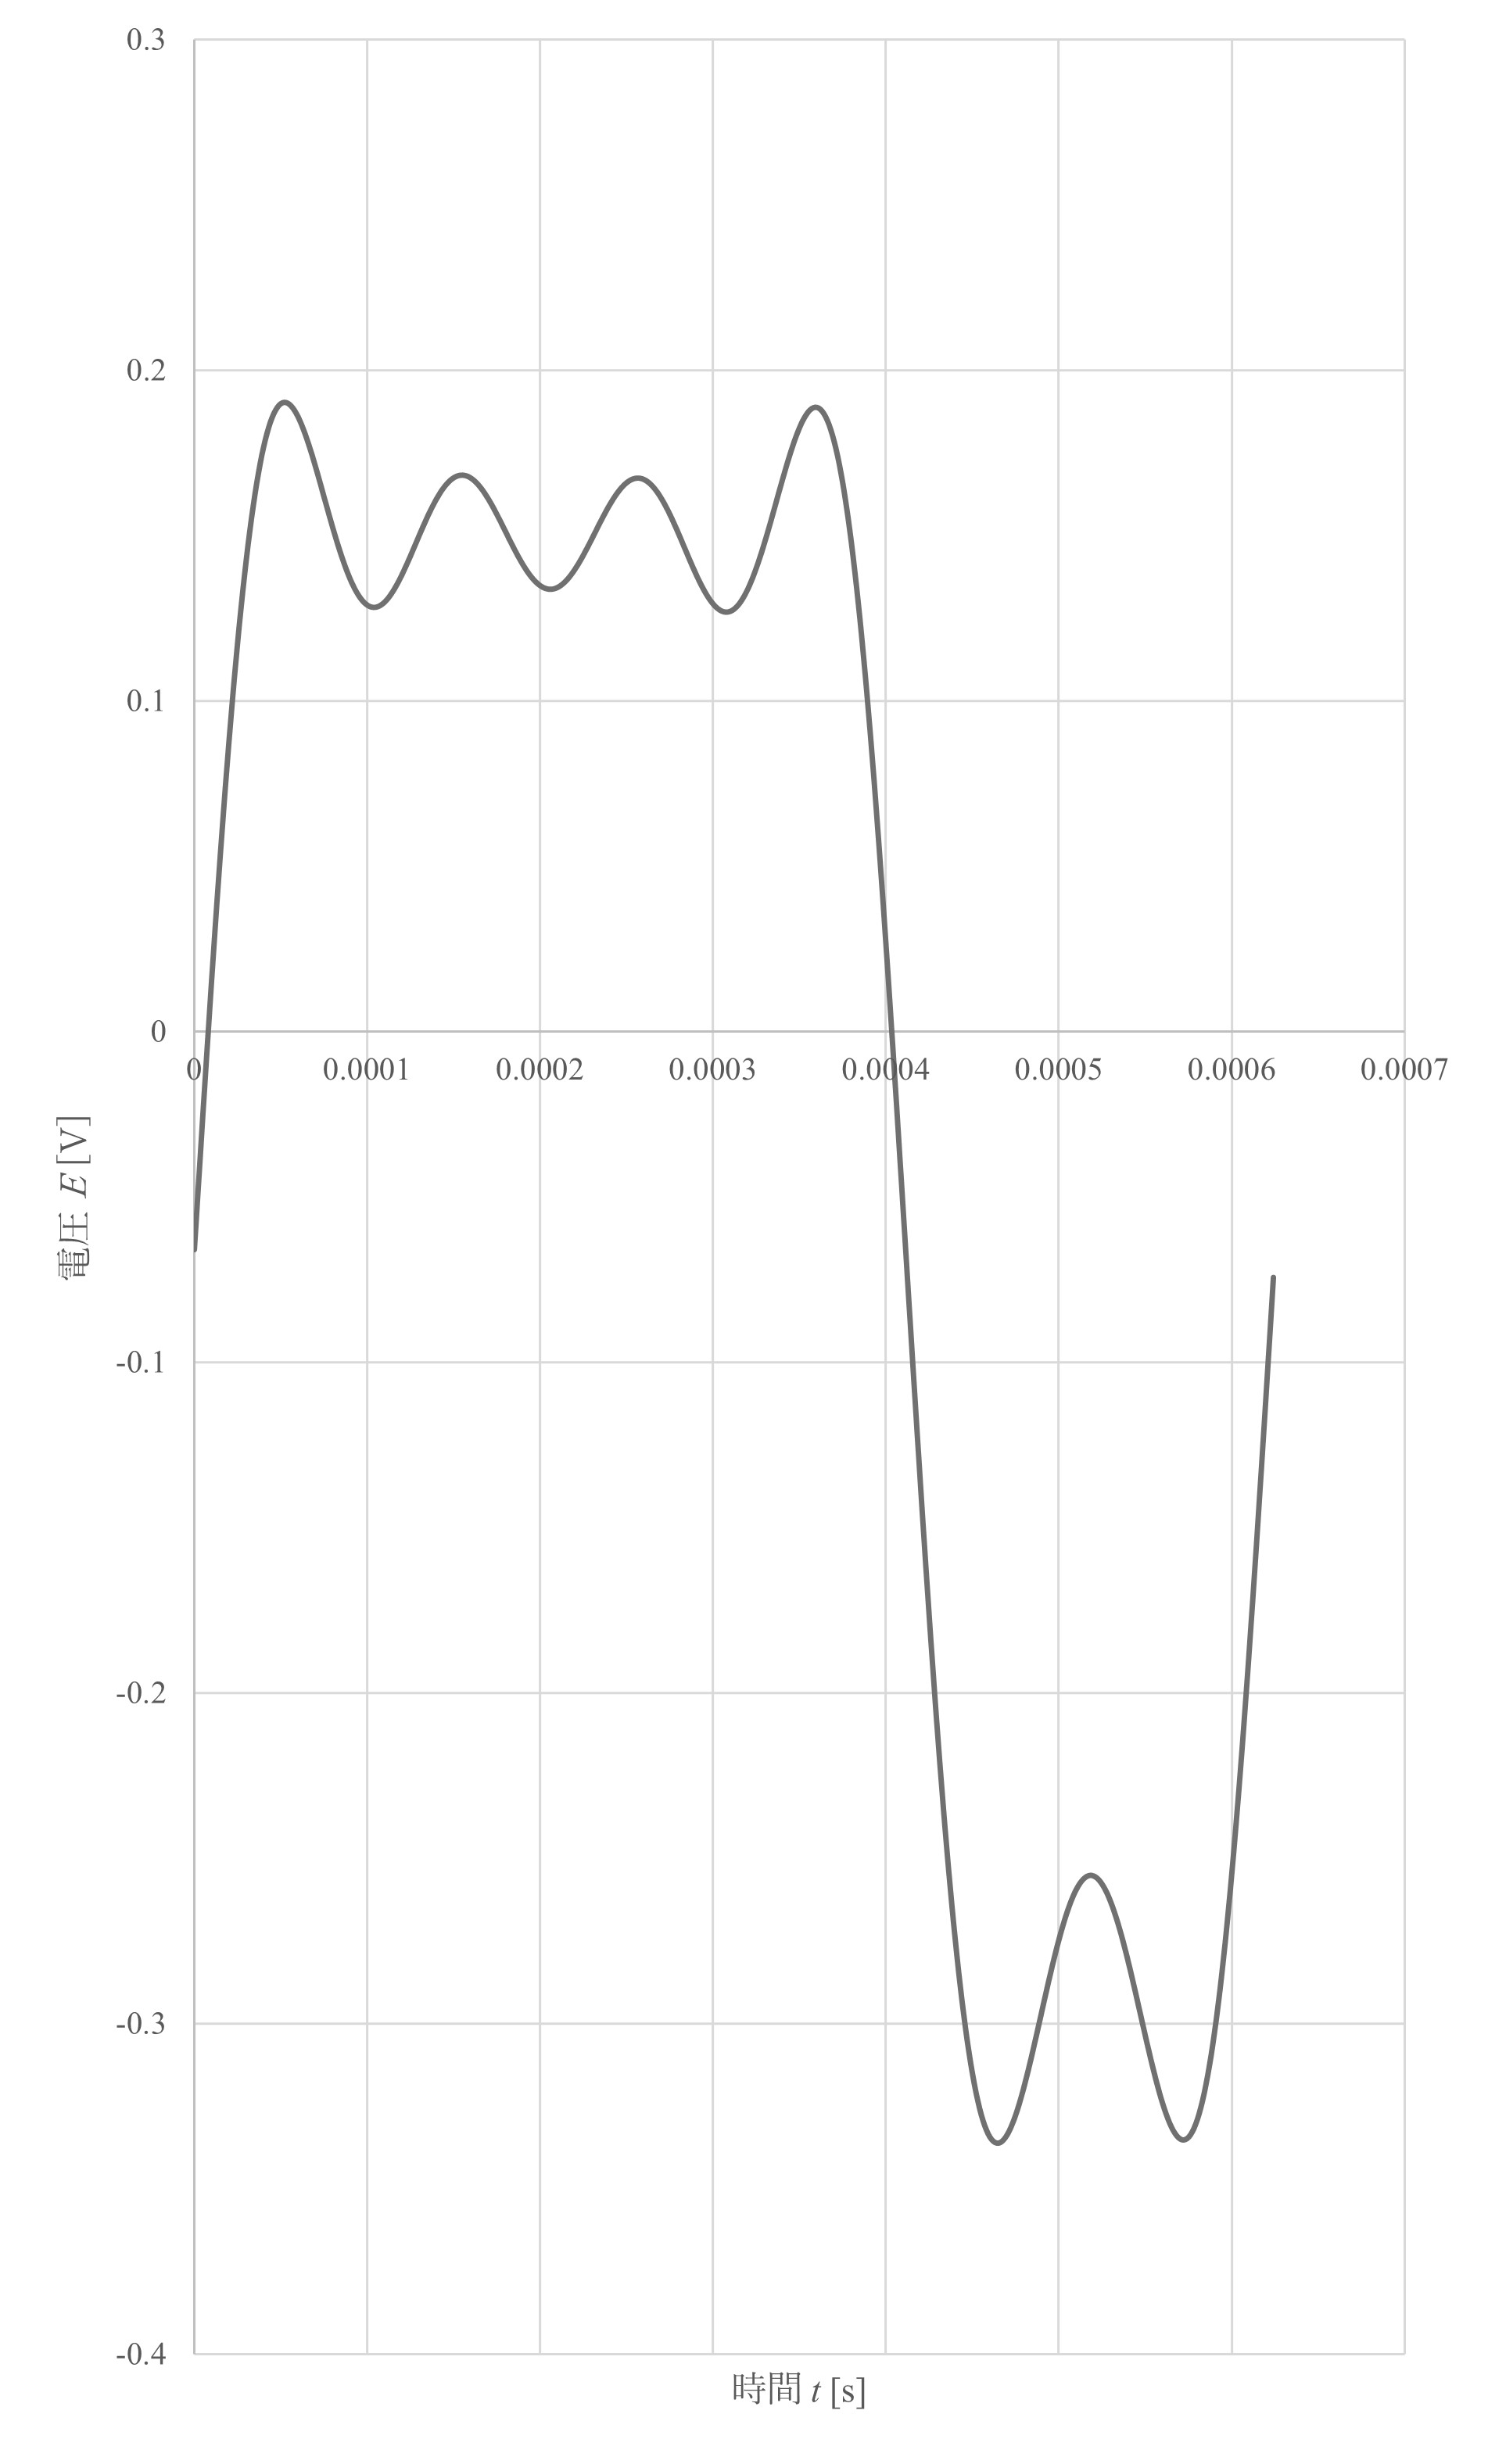
\includegraphics[width=.4\columnwidth]{img/9.jpg}
      \label{sub5}
    }
    \subfigure[被測定波形]{
    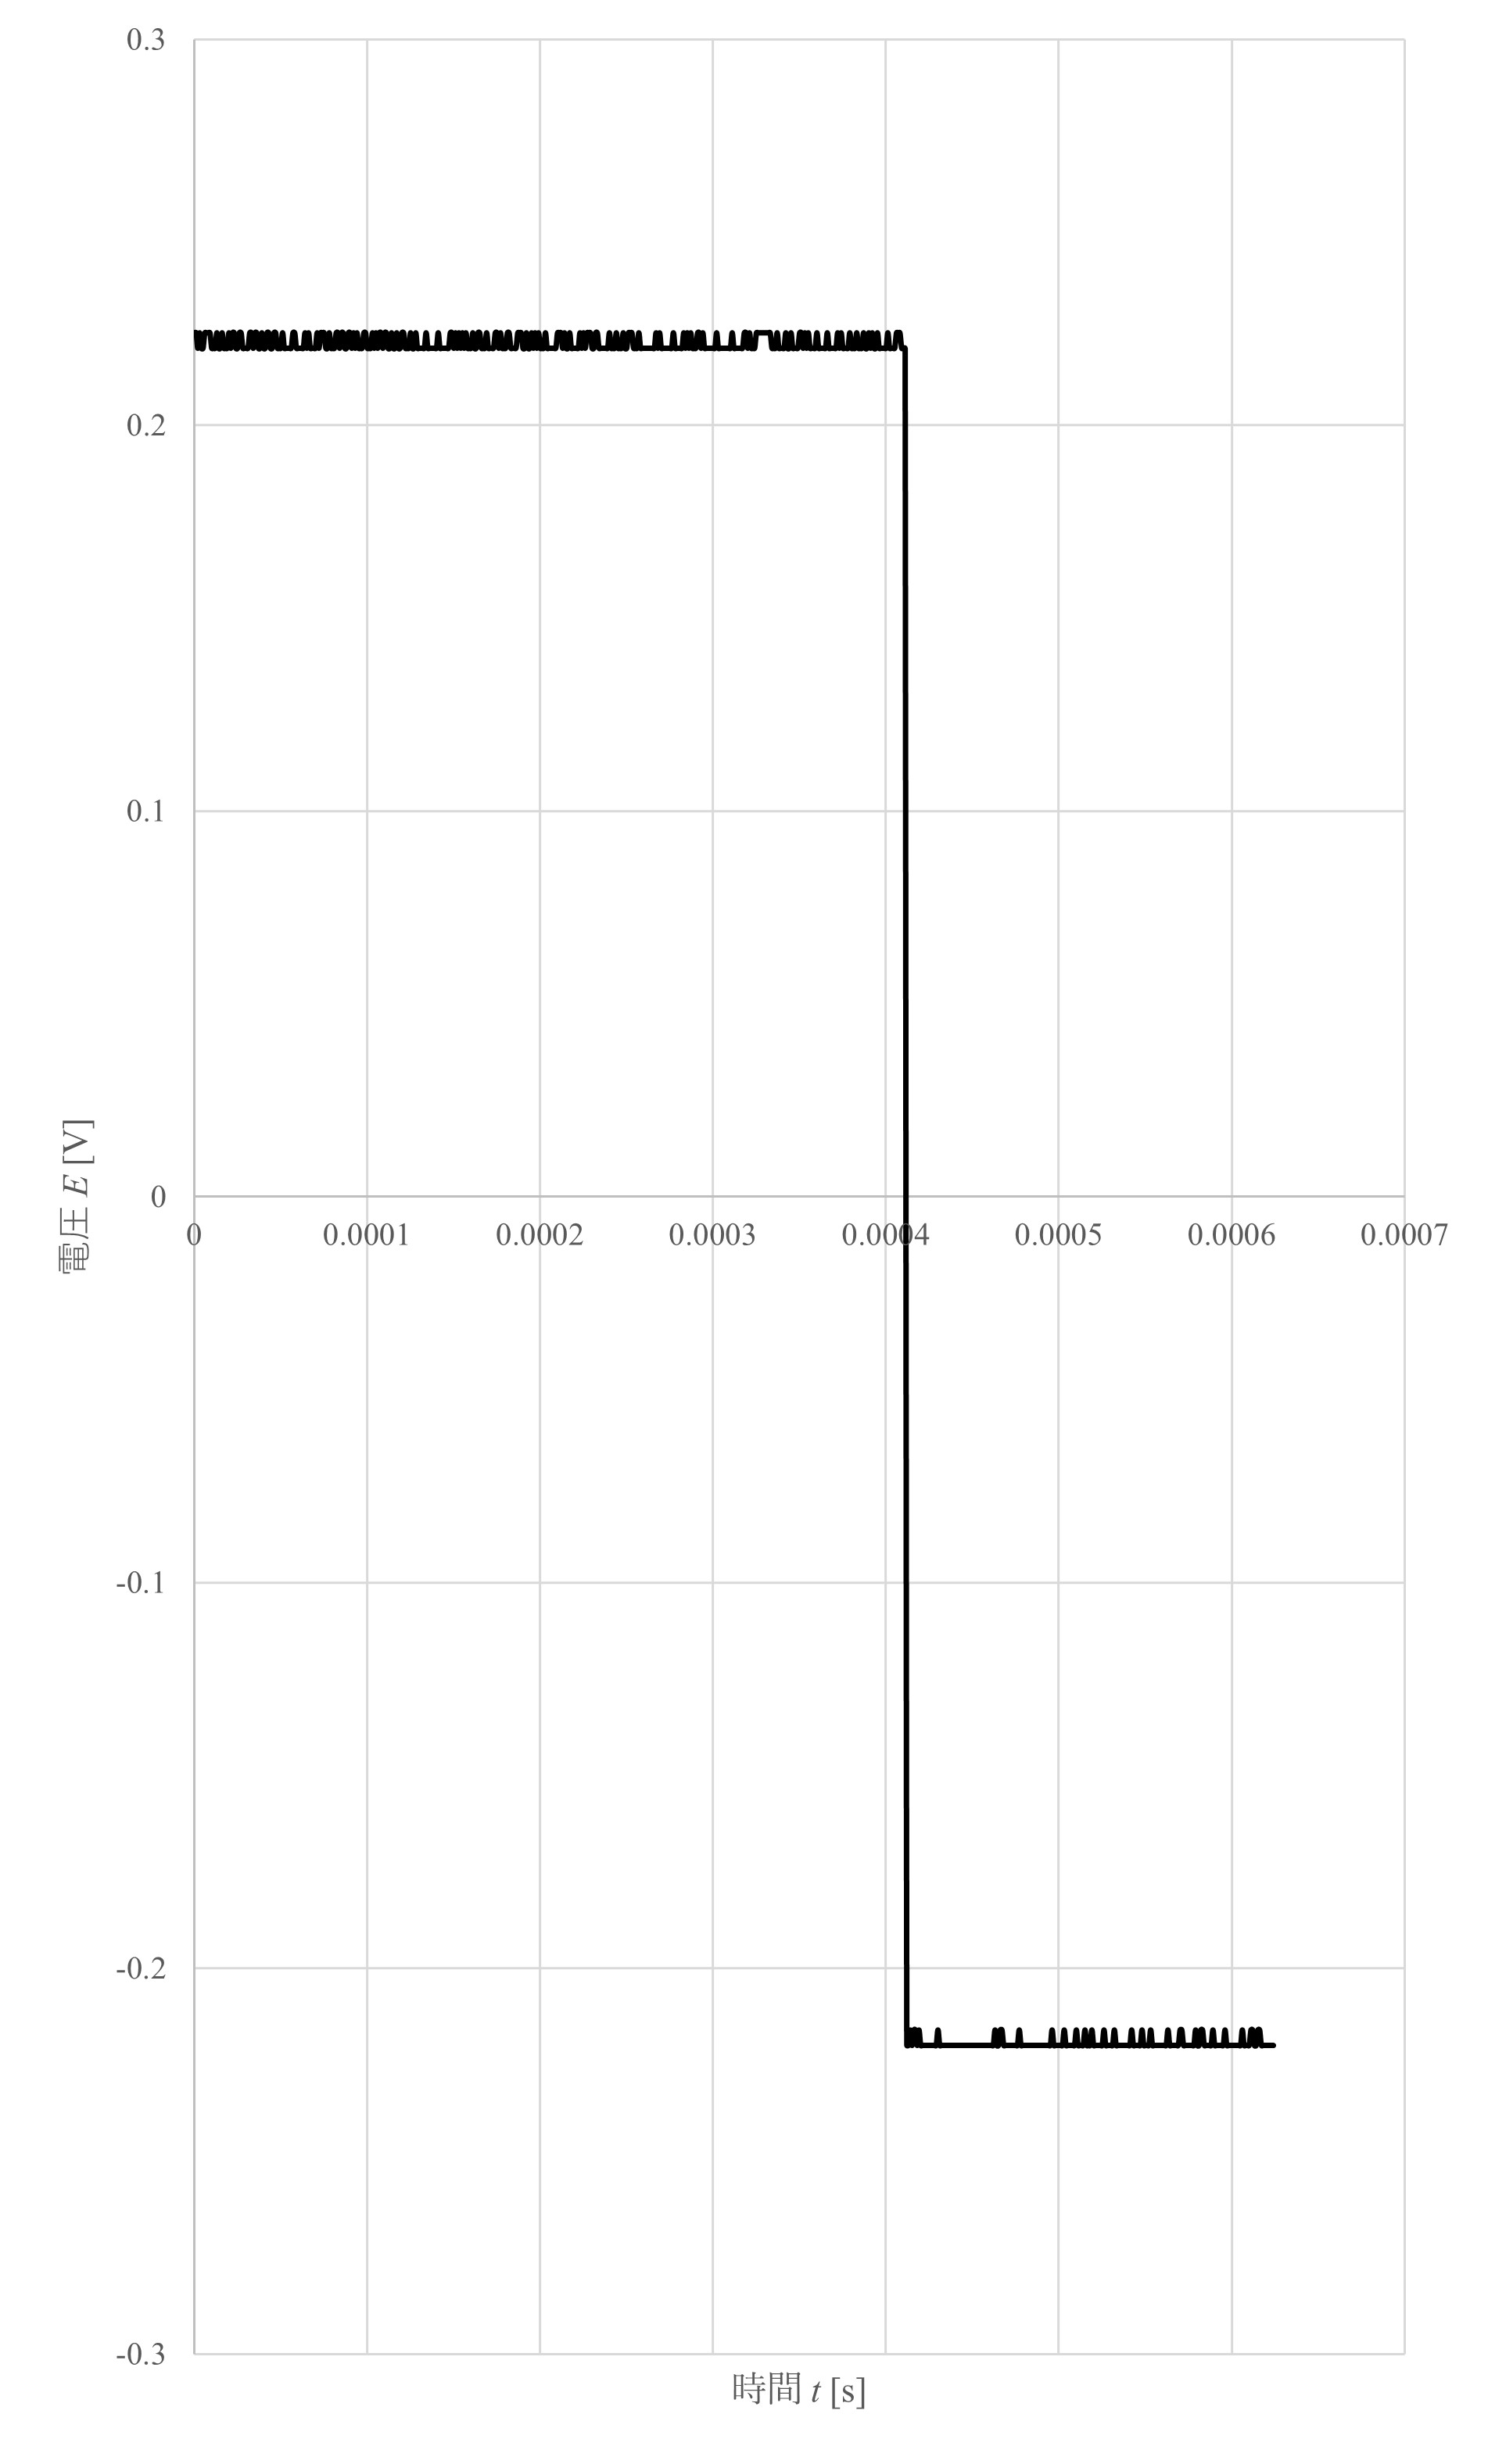
\includegraphics[width=.4\columnwidth]{img/10.jpg}
      \label{sub6}
    }~
    \subfigure[フーリエ級数展開の定義式による波形近似($n = 6$まで)]{
    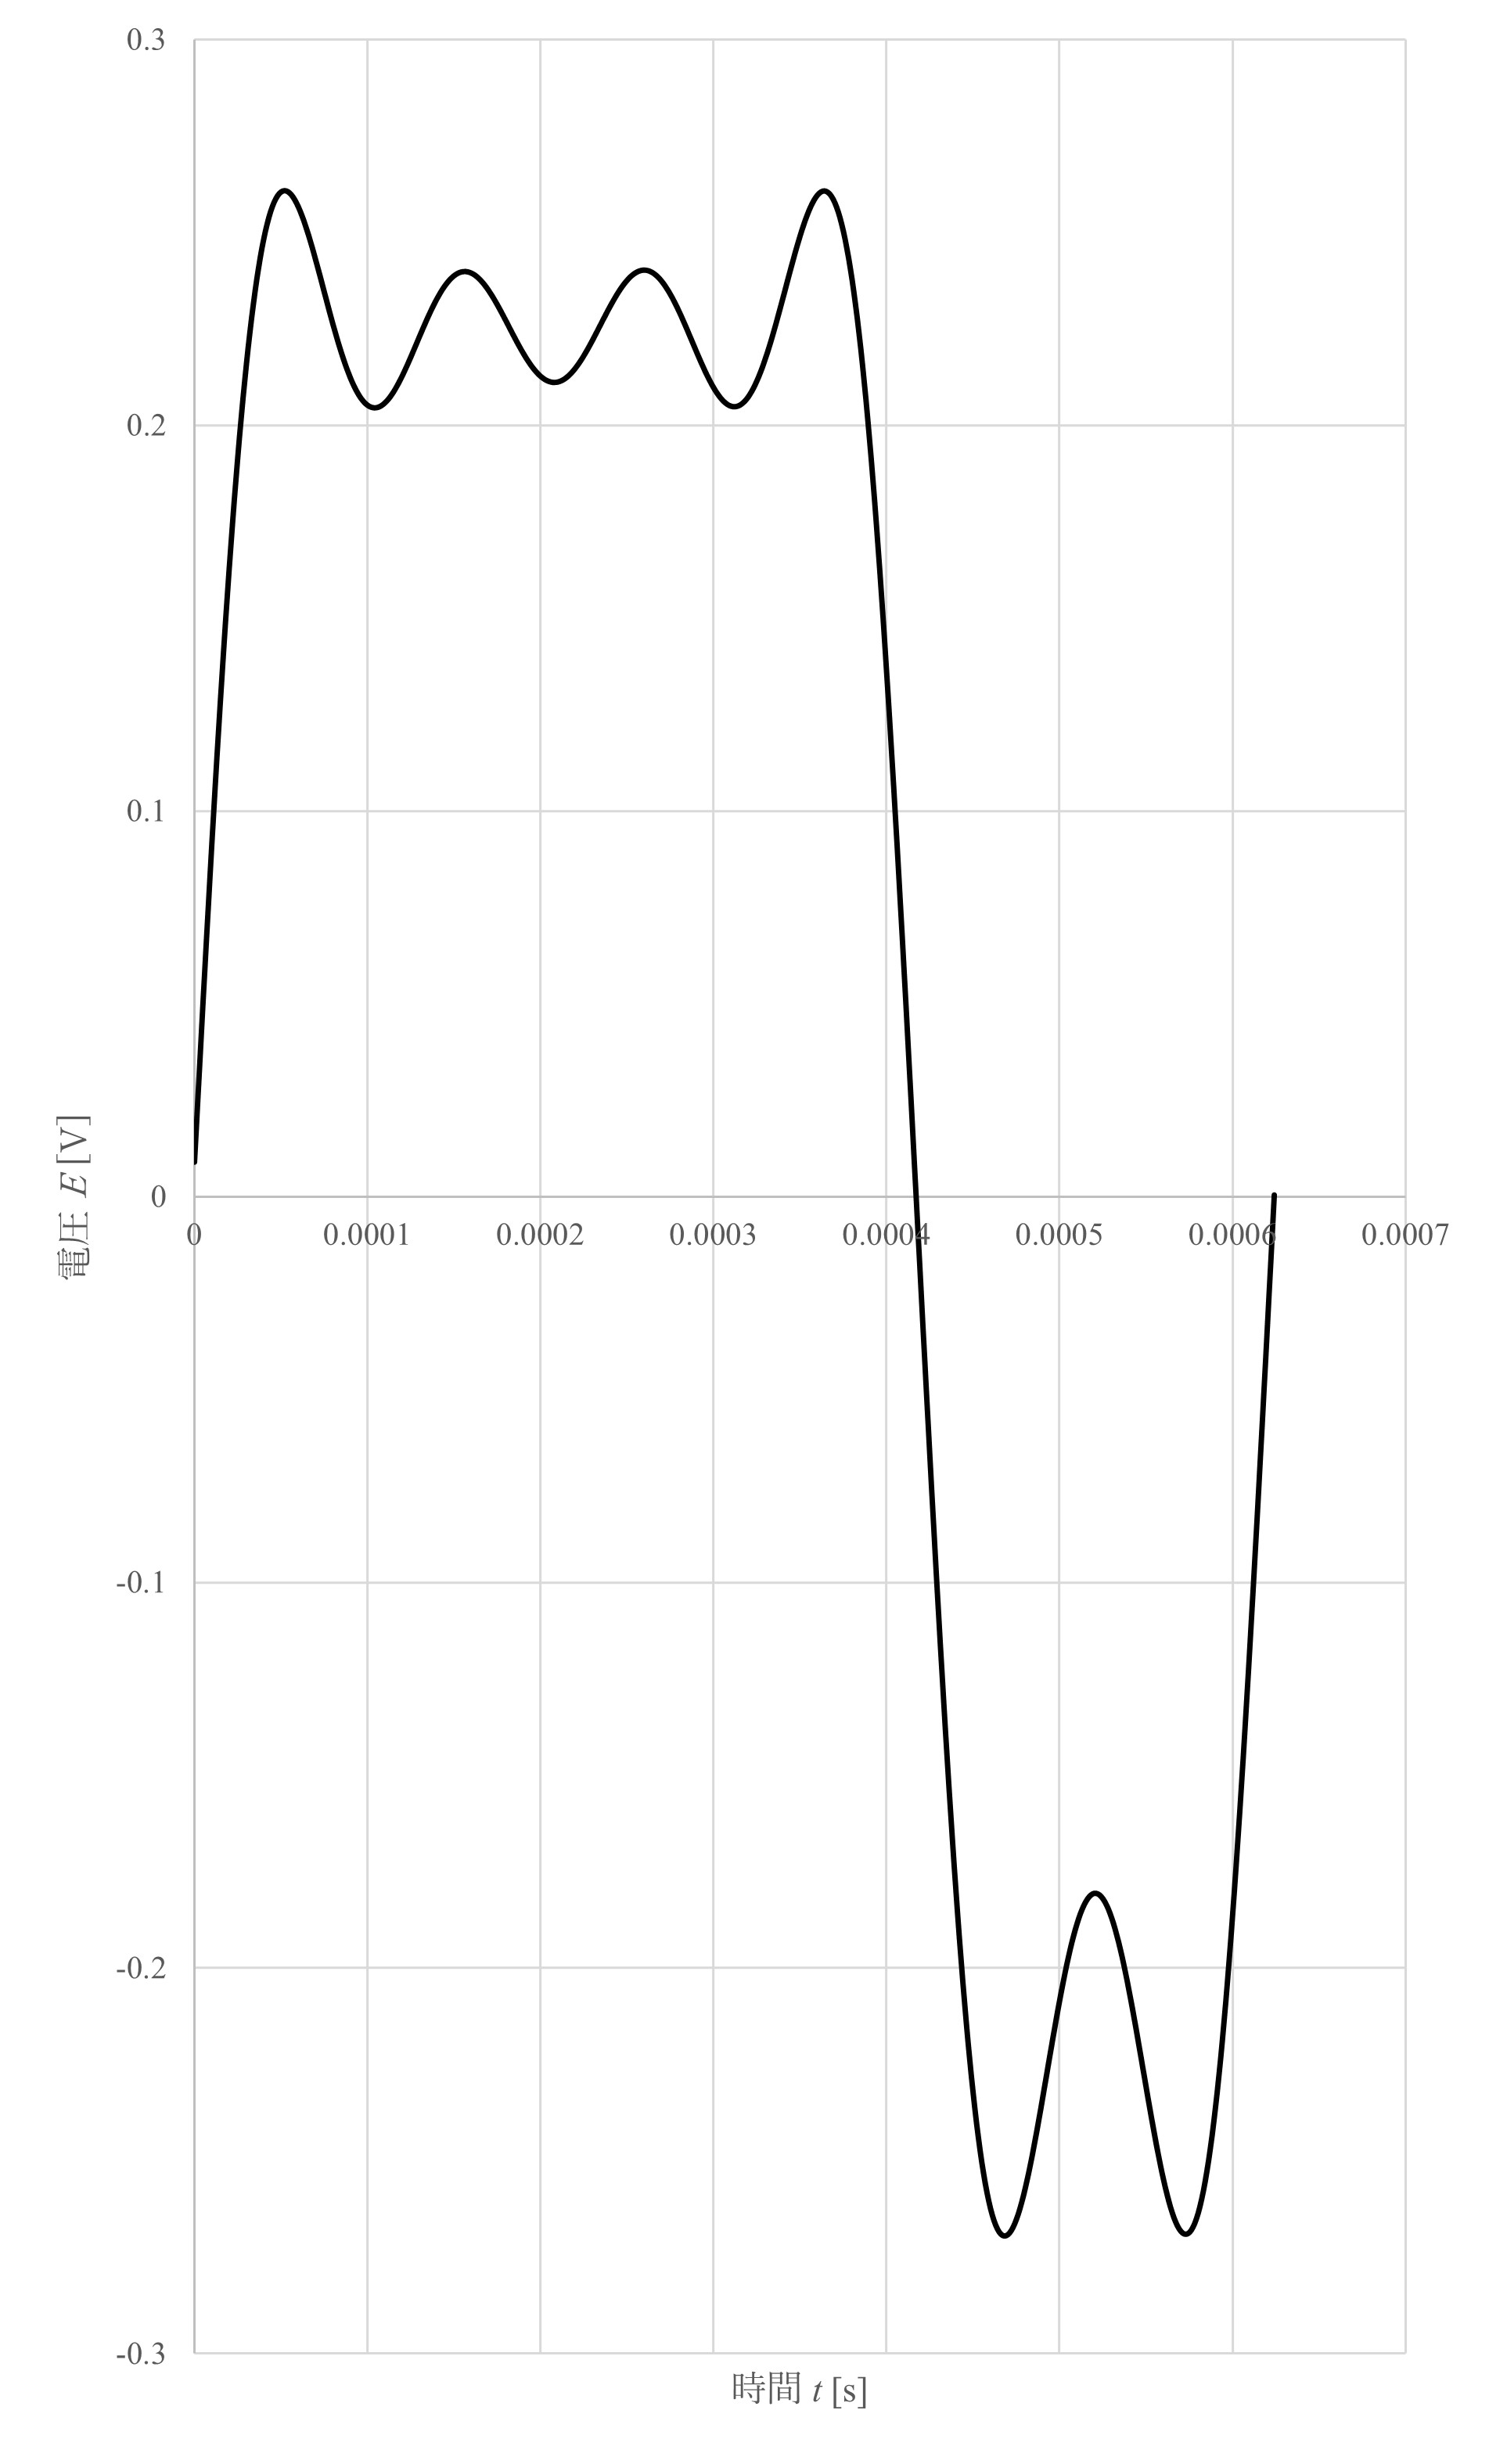
\includegraphics[width=.4\columnwidth]{img/11.jpg}
      \label{sub7}
    }
   \caption{フーリエ級数による近似}
   \label{im6}
   \end{center}
\end{figure}

実験 (14) の結果について、図\ref{im6} \subref{sub6}より、
\begin{screen}
  \begin{equation}
    f(t) = \left\{
      \begin{array}{ll}
        225 \si{[\milli V]} & (0 \leqq t < t \si{[s]})\\
        -220 \si{[\milli V]} & (0.000416 \leqq t < 0.000625 \si{[s]})\\
      \end{array}
      \right.
      \label{eq7}
    \end{equation}
\end{screen}

実験 (15) の結果について式\ref{eq2} \verb|~| \ref{eq4} によってフーリエ係数を計算した過程と結果を、
式\ref{eq9} ~ 式\ref{eq20}表\ref{tb5}, \ref{tb6} に示す。
フーリエ級数展開の有効数字について、式\ref{eq3}, \ref{eq4} の計算は、時間関数と三角関数の積で、時間関数の位取りは3桁で三角関数の位取りは9桁となっているから、
積において位取りの少ない方に有効桁を合わせるため、有効桁を3桁とする。
(角度はラジアンで計算、周期$T = 1/1600 \si{[s]} $)

\begin{screen}
\begin{equation}
  \begin{aligned}
    b_0 &= 1600\times\left\{ \int_{0}^{0.000416}0.225 \,dt+ \int_{0.000416}^{0.000625}-0.220 \,dt \right\}\\
    &= 1600\times\left\{ \left[0.225t\right]^{0.000416}_0+ \left[-0.220t\right]^{0.000625}_{0.000416} \right\} \approx 0.0762 \si{[V]} \label{eq8} 
  \end{aligned}
\end{equation}
\end{screen}

\begin{screen}
  \begin{equation}
    \begin{aligned}
      b_1 &= 2\times1600\times\left\{ \int_{0}^{0.000416}0.225\cos 3200\pi t \,dt+ \int_{0.000416}^{0.000625}-0.220\cos 3200\pi t \,dt \right\}\\
      &= 2\times1600\times\left\{ \left[0.225\frac{\sin3200\pi t}{3200\pi}\right]^{0.000416}_0+ \left[-0.220\frac{\sin 3200\pi t}{3200\pi}\right]^{0.000625}_{0.000416} \right\} \approx -0.122 \si{[V]} \label{eq9}
    \end{aligned}
  \end{equation}
\end{screen}

\begin{screen}
  \begin{equation}
    \begin{aligned}
      b_2 &= 2\times1600\times\left\{ \int_{0}^{0.000416}0.225\cos 6400\pi t \,dt+ \int_{0.000416}^{0.000625}-0.220\cos 6400\pi t \,dt \right\}\\
      &= 2\times1600\times\left\{ \left[0.225\frac{\sin6400\pi t}{6400\pi}\right]^{0.000416}_0+ \left[-0.220\frac{\sin 6400\pi t}{6400\pi}\right]^{0.000625}_{0.000416} \right\} \approx 0.0618 \si{[V]} \label{eq10}
    \end{aligned}
  \end{equation}
\end{screen}

\begin{screen}
  \begin{equation}
    \begin{aligned}
      b_3 &= 2\times1600\times\left\{ \int_{0}^{0.000416}0.225\cos 9600\pi t \,dt+ \int_{0.000416}^{0.000625}-0.220\cos 9600\pi t \,dt \right\}\\
      &= 2\times1600\times\left\{ \left[0.225\frac{\sin9600\pi t}{9600\pi}\right]^{0.000416}_0+ \left[-0.220\frac{\sin 9600\pi t}{9600\pi}\right]^{0.000625}_{0.000416} \right\} \approx -0.000949 \si{[V]} \label{eq11}
    \end{aligned}
  \end{equation}
\end{screen}

\begin{screen}
  \begin{equation}
    \begin{aligned}
      b_4 &= 2\times1600\times\left\{ \int_{0}^{0.000416}0.225\cos 12800\pi t \,dt+ \int_{0.000416}^{0.000625}-0.220\cos 12800\pi t \,dt \right\}\\
      &= 2\times1600\times\left\{ \left[0.225\frac{\sin12800\pi t}{12800\pi}\right]^{0.000416}_0+ \left[-0.220\frac{\sin 12800\pi t}{12800\pi}\right]^{0.000625}_{0.000416} \right\} \approx -0.0302 \si{[V]} \label{eq12}
    \end{aligned}
  \end{equation}
\end{screen}

\begin{screen}
  \begin{equation}
    \begin{aligned}
      b_5 &= 2\times1600\times\left\{ \int_{0}^{0.000416}0.225\cos 16000\pi t \,dt+ \int_{0.000416}^{0.000625}-0.220\cos 16000\pi t \,dt \right\}\\
      &= 2\times1600\times\left\{ \left[0.225\frac{\sin16000\pi t}{16000\pi}\right]^{0.000416}_0+ \left[-0.220\frac{\sin 16000\pi t}{16000\pi}\right]^{0.000625}_{0.000416} \right\} \approx 0.0250 \si{[V]} \label{eq13}
    \end{aligned}
  \end{equation}
\end{screen}

\begin{screen}
  \begin{equation}
    \begin{aligned}
      b_6 &= 2\times1600\times\left\{ \int_{0}^{0.000416}0.225\cos 19200\pi t \,dt+ \int_{0.000416}^{0.000625}-0.220\cos 19200\pi t \,dt \right\}\\
      &= 2\times1600\times\left\{ \left[0.225\frac{\sin192000\pi t}{19200\pi}\right]^{0.000416}_0+ \left[-0.220\frac{\sin 19200\pi t}{19200\pi}\right]^{0.000625}_{0.000416} \right\} \approx -0.000949 \si{[V]} \label{eq14}
    \end{aligned}
  \end{equation}
\end{screen}

\begin{screen}
  \begin{equation}
    \begin{aligned}
      a_1 &= 2\times1600\times\left\{ \int_{0}^{0.000416}0.225\sin 3200\pi t \,dt+ \int_{0.000416}^{0.000625}-0.220\sin 3200\pi t \,dt \right\}\\
      &= 2\times1600\times\left\{ \left[0.225\frac{\cos3200\pi t}{3200\pi}\right]^{0.000416}_0+ \left[-0.220\frac{\cos 3200\pi t}{3200\pi}\right]^{0.000625}_{0.000416} \right\} \approx 0.213 \si{[V]} \label{eq15}
    \end{aligned}
  \end{equation}
\end{screen}

\begin{screen}
  \begin{equation}
    \begin{aligned}
      a_2 &= 2\times1600\times\left\{ \int_{0}^{0.000416}0.225\sin 6400\pi t \,dt+ \int_{0.000416}^{0.000625}-0.220\sin 6400\pi t \,dt \right\}\\
      &= 2\times1600\times\left\{ \left[0.225\frac{\cos6400\pi t}{6400\pi}\right]^{0.000416}_0+ \left[-0.220\frac{\cos 6400\pi t}{6400\pi}\right]^{0.000625}_{0.000416} \right\} \approx 0.105 \si{[V]} \label{eq16}
    \end{aligned}
  \end{equation}
\end{screen}

\begin{screen}
  \begin{equation}
    \begin{aligned}
      a_3 &= 2\times1600\times\left\{ \int_{0}^{0.000416}0.225\sin 9600\pi t \,dt+ \int_{0.000416}^{0.000625}-0.220\sin 9600\pi t \,dt \right\}\\
      &= 2\times1600\times\left\{ \left[0.225\frac{\cos9600\pi t}{9600\pi}\right]^{0.000416}_0+ \left[-0.220\frac{\cos 9600\pi t}{9600\pi}\right]^{0.000625}_{0.000416} \right\} \approx 0.00000954 \si{[V]} \label{eq17}
    \end{aligned}
  \end{equation}
\end{screen}

\begin{screen}
  \begin{equation}
    \begin{aligned}
      a_4 &= 2\times1600\times\left\{ \int_{0}^{0.000416}0.225\sin 12800\pi t \,dt+ \int_{0.000416}^{0.000625}-0.220\sin 12800\pi t \,dt \right\}\\
      &= 2\times1600\times\left\{ \left[0.225\frac{\cos12800\pi t}{12800\pi}\right]^{0.000416}_0+ \left[-0.220\frac{\cos 12800\pi t}{12800\pi}\right]^{0.000625}_{0.000416} \right\} \approx 0.0539 \si{[V]} \label{eq18}
    \end{aligned}
  \end{equation}
\end{screen}

\begin{screen}
  \begin{equation}
    \begin{aligned}
      a_5 &= 2\times1600\times\left\{ \int_{0}^{0.000416}0.225\sin 16000\pi t \,dt+ \int_{0.000416}^{0.000625}-0.220\sin 16000\pi t \,dt \right\}\\
      &= 2\times1600\times\left\{ \left[0.225\frac{\cos16000\pi t}{16000\pi}\right]^{0.000416}_0+ \left[-0.220\frac{\cos 16000\pi t}{16000\pi}\right]^{0.000625}_{0.000416} \right\} \approx 0.0417 \si{[V]} \label{eq19}
    \end{aligned}
  \end{equation}
\end{screen}

\begin{screen}
  \begin{equation}
    \begin{aligned}
      a_6 &= 2\times1600\times\left\{ \int_{0}^{0.000416}0.225\sin 19200\pi t \,dt+ \int_{0.000416}^{0.000625}-0.220\sin 19200\pi t \,dt \right\}\\
      &= 2\times1600\times\left\{ \left[0.225\frac{\cos19200\pi t}{19200\pi}\right]^{0.000416}_0+ \left[-0.220\frac{\cos 19200\pi t}{19200\pi}\right]^{0.000625}_{0.000416} \right\} \approx 0.0000191 \si{[V]} \label{eq20}
    \end{aligned}
  \end{equation}
\end{screen}

\begin{table}[h]
  \begin{center}
    \begin{tabular}{cc}
      \begin{minipage}{0.45\textwidth}
        \centering
        \caption{フーリエ級数$b_n$について}
        \begin{tabular}[t]{rr}
          \toprule
          \multicolumn{1}{c}{$b_n$}&\multicolumn{1}{c}{フーリエ級数の値 \si{[V]}}\\
          \midrule
          $b_0$&0.0762\\
          $b_1$&-0.122\\
          $b_2$&0.0618\\
          $b_3$&-0.000949\\
          $b_4$&-0.0302\\
          $b_5$&0.0250\\
          $b_6$&-0.000949\\
          \bottomrule
        \end{tabular}
        \label{tb5}
      \end{minipage}
      \begin{minipage}{0.4\textwidth}
        \centering
        \caption{フーリエ級数$a_n$について}
        \begin{tabular}[t]{rr}
          \toprule
          \multicolumn{1}{c}{$a_n$}&\multicolumn{1}{c}{フーリエ級数の値 \si{[V]}}\\
          \midrule
          $a_1$&0.213\\
          $a_2$&0.105\\
          $a_3$&0.00000954\\
          $a_4$&0.0539\\
          $a_5$&0.0417\\
          $a_6$&0.000191\\
          \bottomrule
        \end{tabular}
        \label{tb6}
      \end{minipage}
    \end{tabular}
  \end{center}
\end{table}